% =====================================================================
% Report for the Natural Language Engineering (NLE) template.
% HOW TO USE: open the "Natural Language Engineering" template on Overleaf,
% keep its \documentclass/preamble lines, and replace everything from
% \title{...} to \end{document} with the content below.
% Needs \usepackage{graphicx} in the preamble and the figures/ folder uploaded to Overleaf.
%
% DRAFT STATUS (21 Nov): all sections that do not depend on the transformer / LLM / LIME runs are drafted.
% Every place that still needs a number or a finding is marked \tbd{...} (prints in bold brackets) or
% "% TODO" (comment only). Search for "\tbd" and "TODO" before submitting; both must be gone.
% Numbers must be copied from results/summary.csv, results/significance.txt and results/analysis/,
% never typed from memory. "% VERIFY" marks a claim about another paper to check against that paper.
% Section tags [writer -> reviewers] show who reviews each section. Remove them before submitting.
% =====================================================================
\providecommand{\tbd}[1]{\textbf{[TBD: #1]}}

\title[Stress Detection with Domain-Adapted Language Models]
      {Stress Detection in Social Media Posts with\\ Domain-Adapted Language Models}
\author[S. Yadav, S. Bisht and S. Mishra]
       {SUYASH YADAV, SAURABH BISHT and SARTHAK MISHRA\\
        Sitare University\\
        \texttt{https://github.com/Iamdevsuyash/stress-detection-dreaddit}}

\begin{document}
\label{firstpage}
\maketitle

\begin{abstract}
% [Sarthak -> Suyash, Saurabh] Written LAST, once all results are in. 150-200 words.
% Skeleton below: keep the structure, fill the brackets from results/summary.csv.
People often describe stress in social media posts before they seek help, so detecting it
automatically could support early, voluntary interventions. We study binary stress detection on
Dreaddit, a corpus of 3,553 crowd-labelled Reddit segments from ten subreddits, and ask whether
language models pretrained on mental-health text outperform general-purpose ones. Using a single
fixed data split, three random seeds and paired significance tests, we compare a BiLSTM with GloVe
embeddings, the general encoders BERT and RoBERTa, their mental-health counterparts MentalBERT and
MentalRoBERTa, and an instruction-tuned LLM (Qwen2.5-7B) used zero- and few-shot without any training.
\tbd{best model and its macro-F1}; domain-adapted pretraining \tbd{helps / does not significantly
help} (\tbd{BERT vs MentalBERT gap, p-value}). The untrained LLM reaches \tbd{macro-F1}, \tbd{x points}
below the best fine-tuned encoder. LIME explanations show that \tbd{main cue finding}. We close with a
discussion of the privacy, harm and dual-use risks of mental-health inference from social media.
\end{abstract}

% =====================================================================
\section{Introduction}
% [Suyash -> Sarthak]
Stress is the experience of facing demands that seem to exceed one's resources to cope with them
\cite{lazarus1984stress}. Short episodes are a normal part of life, but sustained stress is linked to
anxiety, depression and physical illness, and many people first put their difficulties into words
online, often long before they contact a professional. Reddit is a natural place to study this:
users write long, pseudonymous posts in topic-specific communities such as r/anxiety,
r/domesticviolence or r/homeless, where they describe their situation in their own words. Models
that recognise stress in such text could help moderators prioritise posts, help researchers measure
population-level well-being, and support opt-in self-monitoring tools. The same models can also be
misused, which we discuss in Section~\ref{sec:ethics}.

Pretrained transformer encoders such as BERT \cite{devlin2019bert} and RoBERTa \cite{liu2019roberta}
are the standard approach to text classification of this kind. They are pretrained on books,
Wikipedia, news and web text, however, while posts about stress are informal, emotional and
written in the first person. Gururangan {\it et al.}~\shortcite{gururangan2020dont} showed that continuing to pretrain a model
on text from the target domain (domain-adaptive pretraining, DAPT) usually improves downstream
performance. MentalBERT and MentalRoBERTa \cite{ji2022mentalbert} apply this idea to mental health:
they continue the pretraining of BERT and RoBERTa on posts from mental-health subreddits. At the
same time, instruction-tuned large language models (LLMs) can classify text from a prompt alone,
with no task-specific training \cite{brown2020language,xu2024mentalllm}, which raises the question of
whether fine-tuning a small encoder is still worth the effort.

This paper compares these approaches under one controlled setup and answers three research questions:
\begin{enumerate}
  \item[\textbf{RQ1}] Does mental-health-domain pretraining (MentalBERT, MentalRoBERTa) improve stress
        detection over general pretraining (BERT, RoBERTa)?
  \item[\textbf{RQ2}] How does an instruction-tuned LLM, used zero-shot or with four examples, compare
        with fine-tuned encoders?
  \item[\textbf{RQ3}] Which words and phrases drive the predictions, and do the general and the
        domain-adapted models rely on different cues?
\end{enumerate}

Our contributions are:
(i) a comparison of four model families on Dreaddit \cite{turcan2019dreaddit}, in which every model
uses the same post-grouped validation split, the same evaluation code and three random seeds, and
the key comparisons are tested with McNemar's test and a paired bootstrap;
(ii) a zero- and few-shot LLM baseline that reads the probability of the answer tokens instead of
parsing generated text, so it never fails to produce a label and its decision threshold can be
tuned on the validation set;
(iii) a LIME-based comparison of the cues used by BERT and MentalBERT, together with an error
analysis by subreddit; and
(iv) a discussion of the ethical risks of inferring mental states from social media.
All code, data splits (as post identifiers), predictions and metrics are public in our repository.

% =====================================================================
\section{Related Work}
% [Suyash (2),(3); Saurabh (1),(4); Sarthak edits]

\paragraph{Stress and mental-health detection on social media.}
% [Saurabh -> Sarthak]
Social media text has been used to detect depression, anxiety, suicidal ideation and other
conditions for more than a decade \cite{coppersmith2014quantifying,guntuku2017detecting}.
Turcan and McKeown~\shortcite{turcan2019dreaddit} released Dreaddit, the first large dataset for stress specifically: 3,553
five-sentence segments from ten subreddits in five domains, each labelled by several crowd workers.
They compared logistic regression with lexical and syntactic features against neural models,
including fine-tuned BERT, and found the two families to be close.
% VERIFY against Turcan and McKeown (2019), Table 7: they report binary F1 for the stress class,
% which corresponds to our "F1 (stress)" column, not macro-F1. Add their best numbers here if quoted.
Dreaddit has since become a standard benchmark for mental-health language models:
Ji {\it et al.}~\shortcite{ji2022mentalbert} use it to evaluate MentalBERT, and Xu {\it et al.}~\shortcite{xu2024mentalllm} and
Yang {\it et al.}~\shortcite{yang2023towards} use it to evaluate prompted and instruction-tuned LLMs.

\paragraph{Pretrained and domain-adapted language models.}
% [Suyash -> Saurabh]
BERT \cite{devlin2019bert} learns contextual representations by masked-language-model pretraining
on BooksCorpus and English Wikipedia; RoBERTa \cite{liu2019roberta} keeps the architecture but trains
longer, on more data (including web and news text), with dynamic masking and without the
next-sentence objective. Gururangan {\it et al.}~\shortcite{gururangan2020dont} showed that a second phase of pretraining on
unlabelled text from the target domain (DAPT) or from the task itself (task-adaptive pretraining,
TAPT) improves performance in domains far from the original pretraining data, such as biomedical
papers and reviews. MentalBERT and MentalRoBERTa \cite{ji2022mentalbert} are DAPT models for mental
health: BERT-base and RoBERTa-base checkpoints further pretrained on posts from mental-health
subreddits.
% VERIFY in Ji et al. (2022), Sec. 3: the exact subreddit list (we believe it includes r/Anxiety,
% which is also a Dreaddit source; if so, mention the possible topical overlap in Limitations).
Instruction-tuned LLMs offer a different route: Brown {\it et al.}~\shortcite{brown2020language} showed that large language
models can perform new tasks from a handful of examples in the prompt, and Xu {\it et al.}~\shortcite{xu2024mentalllm}
found that prompted LLMs are competitive on some mental-health tasks but generally trail fine-tuned
models.

\paragraph{Explaining model predictions.}
% [Suyash -> Saurabh]
LIME \cite{ribeiro2016lime} explains a single prediction of any black-box classifier by perturbing
the input (for text, deleting words) and fitting a sparse linear model to the classifier's outputs on
the perturbed samples; the weights of that local model indicate how much each word pushed the
prediction. Attention weights are a cheaper alternative for transformers, but
Jain and Wallace~\shortcite{jain2019attention} showed that they often do not agree with gradient-based importance and that
different attention patterns can yield the same prediction, while Wiegreffe and Pinter~\shortcite{wiegreffe2019attention}
argued that attention can still be informative under some conditions. We therefore treat LIME as our
primary explanation method and show attention only as an illustration.

\paragraph{Ethics of mental-health NLP.}
% [Saurabh -> Sarthak]
Benton {\it et al.}~\shortcite{benton2017ethical} proposed research protocols for social-media health research, including
de-identification, restricted data sharing and review by an ethics board.
Chancellor {\it et al.}~\shortcite{chancellor2019taxonomy} described tensions specific to inferring mental-health states from
social media: whether the predicted construct is valid, who benefits, and the risks of
false positives, false negatives and surveillance. Conway and O'Connor~\shortcite{conway2016social} reviewed the ethical
implications of using social media data for mental-health research. We follow their recommendations
in Section~\ref{sec:ethics}.

% =====================================================================
\section{Dataset}
\label{sec:data}
% [Saurabh -> Suyash]
We use Dreaddit \cite{turcan2019dreaddit}. Its authors collected posts from ten subreddits grouped
into five domains: abuse, anxiety, financial need, post-traumatic stress disorder (PTSD) and social
relationships (Table~\ref{tab:subreddits}). Each post was cut into segments of five sentences, and
each segment was labelled by crowd workers on Amazon Mechanical Turk as \emph{stress} or
\emph{not stress}; the final label is the majority vote. The dataset provides an agreement score per
segment (the fraction of annotators who chose the majority label), which averages 0.79, so many
segments are genuinely ambiguous. In total there are 3,553 labelled segments, 52.3\% of them labelled
\emph{stress}. Segments are short (85 words on average, at most 310), and a single post can contribute
several segments.

\paragraph{Splits.} Dreaddit comes with an official training set (2,838 segments) and test set (715
segments) that share no posts. It has no validation set, so we hold out 10\% of the training set
for model selection. Because segments from the same post are highly similar, a random split would
leak information between training and validation and make validation scores optimistic. We
therefore split by post: all segments of a post go to the same side, using a stratified group
$k$-fold split ($k=10$, seed 42) and taking one fold as validation. The resulting sizes are given in
Table~\ref{tab:splits}. The identifiers of the validation posts are stored in our repository, so the
split is identical on every machine; we never redistribute the post text itself. All models use
exactly this split, every model is selected on the validation set only, and each trained model is
evaluated once on the test set.

\begin{table}
  \caption{Data splits. The validation set is held out from the official training set by Reddit post.}
  \label{tab:splits}
  \begin{minipage}{\textwidth}
  \begin{tabular}{lrrr}
  \hline\hline
  Split & Segments & Posts & \% stress\\
  \hline
  Train      & 2,555 & 2,108 & 52.4\\
  Validation &   283 &   235 & 52.3\\
  Test       &   715 &   586 & 51.6\\
  \hline\hline
  \end{tabular}
  \end{minipage}
\end{table}

\begin{table}
  \caption{Subreddits in Dreaddit, with the number of segments per split and the share labelled
  \emph{stress} across all splits.}
  \label{tab:subreddits}
  \begin{minipage}{\textwidth}
  \begin{tabular}{llrrrr}
  \hline\hline
  Domain & Subreddit & Train & Val & Test & \% stress\\
  \hline
  Abuse     & r/domesticviolence & 277 & 39 &  72 & 64.2\\
            & r/survivorsofabuse & 216 & 29 &  70 & 45.4\\
  Anxiety   & r/anxiety          & 466 & 37 & 147 & 64.0\\
            & r/stress           &  60 &  4 &  14 & 57.7\\
  Financial & r/almosthomeless   &  70 & 10 &  19 & 59.6\\
            & r/assistance       & 252 & 37 &  66 & 35.5\\
            & r/food\_pantry     &  33 &  4 &   6 & 39.5\\
            & r/homeless         & 148 & 20 &  52 & 36.8\\
  PTSD      & r/ptsd             & 522 & 62 & 127 & 58.2\\
  Social    & r/relationships    & 511 & 41 & 142 & 44.2\\
  \hline
  Total     &                    & 2,555 & 283 & 715 & 52.3\\
  \hline\hline
  \end{tabular}
  \end{minipage}
\end{table}

The share of stressed segments varies widely across communities, from about 36\% in the financial
subreddits r/assistance and r/homeless to 64\% in r/anxiety and r/domesticviolence. A model could
partly exploit this by learning the topic rather than the author's state, which we check with the
per-subreddit analysis in Section~\ref{sec:explain}.

% =====================================================================
\section{Methods}
\label{sec:methods}
All models solve the same task: given a segment, predict \emph{stress} (1) or \emph{not stress} (0).

\subsection{BiLSTM with GloVe}
% [Sarthak -> Suyash]
Our non-pretrained baseline is a bidirectional LSTM \cite{hochreiter1997lstm}. Text is lowercased
and split into words and punctuation; the vocabulary contains every training-set token that occurs
at least twice, and segments are cut to 200 tokens. Tokens are embedded with 100-dimensional GloVe
vectors \cite{pennington2014glove} (6B-token version), which are fine-tuned during training; words
without a GloVe vector are initialised randomly. A single-layer BiLSTM with 128 hidden units per
direction reads the sequence, and the outputs at all positions are summarised by concatenating their
element-wise maximum and mean (padding excluded). After dropout (0.5), a linear layer produces the
two class scores. To measure what pretrained word vectors contribute, we also train the same model
with randomly initialised embeddings (\emph{random-embedding ablation}).

\subsection{General pretrained encoders}
% [Suyash -> Saurabh]
We fine-tune BERT-base (uncased) \cite{devlin2019bert} and RoBERTa-base \cite{liu2019roberta}, both
with 12 layers, hidden size 768 and about 110M and 125M parameters respectively. Following standard
practice, a linear classification layer is placed on top of the final representation of the first
token ([CLS] for BERT, \texttt{<s>} for RoBERTa), and all weights are updated with a cross-entropy
loss. Inputs are cut to 256 subword tokens, which truncates only the longest segments.

\subsection{Domain-adapted encoders}
% [Saurabh -> Sarthak]
MentalBERT and MentalRoBERTa \cite{ji2022mentalbert} have exactly the same architecture and tokenizer
as BERT-base and RoBERTa-base; they differ only in a further phase of masked-language-model
pretraining on posts from mental-health subreddits. We fine-tune them with the same classifier and
hyper-parameters as their general counterparts, so each pair (BERT vs MentalBERT, RoBERTa vs
MentalRoBERTa) differs only in the pretraining data. This isolates the effect of domain-adaptive
pretraining, which is the comparison behind RQ1.
% TODO (Saurabh): if the TAPT/DAPT stretch run was done, describe it here: BERT-base further pretrained
% with masked LM (15% masking, 3 epochs, lr 5e-5) on Dreaddit TRAINING text only, then fine-tuned as
% above (tag bert-dapt). Call it TAPT, not DAPT (Gururangan et al. terminology). Otherwise delete.

\subsection{Zero- and few-shot LLM}
% [Sarthak -> Suyash]
As an untrained baseline we prompt Qwen2.5-7B-Instruct \cite{qwen2024qwen25}, an open-weight
instruction-tuned LLM, loaded with 4-bit NF4 quantisation \cite{dettmers2023qlora} so that it fits on
a single 16\,GB GPU. The prompt, given in the model's chat format, is:

\begin{quote}\small
\textit{You will read a short post from Reddit. Decide whether the author of the post is expressing
stress, i.e. they feel overwhelmed, anxious, under pressure, or unable to cope with a situation.
Answer with a single word: Yes or No.\\[2pt]
Post: """\{segment\}"""\\[2pt]
Is the author stressed?}
\end{quote}

\noindent Rather than generating an answer and parsing it, we run one forward pass and read the
model's next-token distribution at the position where the answer would begin. We sum the
probabilities of the tokens that start the answer \emph{Yes} (with and without a leading space or
capital letter) and likewise for \emph{No}, and use the log-odds
$s = \log P(\textit{Yes}) - \log P(\textit{No})$ as the stress score. This has three advantages: every
post receives a valid label, the score supports ROC-AUC, and the decision threshold can be moved.
We work with log-odds rather than $P(\textit{Yes} \mid \textit{Yes or No}) = \sigma(s)$ because the
probability rounds to exactly 1.0 for many posts, which creates ties; the log-odds keep the ranking.

We evaluate two settings. In the \emph{zero-shot} setting the model sees only the instruction and
the segment. In the \emph{4-shot} setting the prompt is preceded by four labelled training segments
(two \emph{stress}, two \emph{not stress}, in random order), presented as earlier user and assistant
turns. Because the result may depend on which examples are shown, the examples are drawn three times
with different seeds. For each setting we report two decision rules: the default threshold $s \ge 0$
(equivalent to $P(\textit{Yes}) \ge 0.5$), and a threshold tuned on the validation set, chosen among
all observed validation scores to maximise macro-F1. The second rule uses 283 labelled examples, so it
is no longer strictly zero-shot, but it shows how much of the gap to fine-tuned models comes from
miscalibration rather than from a lack of understanding.

\subsection{Explanation methods}
% [Saurabh -> Sarthak]
To answer RQ3 we explain the seed-13 BERT and MentalBERT classifiers with LIME
\cite{ribeiro2016lime}. For each of 100 test segments, sampled with the same class balance as the
test set, LIME generates 500 perturbed versions of the segment by removing random subsets of words,
records the classifier's probability of \emph{stress} for each, and fits a weighted linear model whose
10 largest weights are kept as the explanation. To obtain a global picture we sum each word's weights
over all 100 segments; words that appear in fewer than three segments are excluded from the summary
figure, so that it shows recurring cues rather than one-off words. As a complementary, model-internal
view we visualise, for four example segments, the attention that the [CLS] token pays to every other
token in the last layer, averaged over the 12 heads. Following Jain and Wallace~\shortcite{jain2019attention}, we read
these heatmaps as illustrations only, not as faithful explanations.

% =====================================================================
\section{Experimental Setup}
\label{sec:setup}
% [Suyash -> Saurabh]
\paragraph{Training.} Table~\ref{tab:hparams} lists the hyper-parameters. The encoders are fine-tuned
with AdamW \cite{loshchilov2019decoupled} (no weight decay on biases and layer-normalisation weights),
a linear learning-rate schedule with 10\% warm-up, gradient clipping at norm 1.0 and fp16 mixed
precision. We train for four epochs, evaluate on the validation set after each epoch and keep the
epoch with the highest validation macro-F1. The BiLSTM is trained with Adam for up to 20 epochs with
early stopping (patience 4) on validation macro-F1. We did not tune hyper-parameters on the test set;
for the encoders we use the values commonly recommended for BERT fine-tuning.

\begin{table}
  \caption{Hyper-parameters. Encoders share one configuration, so that each general/domain pair
  differs only in its pretraining data.}
  \label{tab:hparams}
  \begin{minipage}{\textwidth}
  \begin{tabular}{lll}
  \hline\hline
  & BiLSTM + GloVe & Encoders (BERT, RoBERTa, Mental-)\\
  \hline
  Optimiser            & Adam             & AdamW, weight decay 0.01\\
  Learning rate        & $10^{-3}$        & $2\times10^{-5}$, linear decay, 10\% warm-up\\
  Batch size           & 32               & 16\\
  Max.\ input length   & 200 words        & 256 subword tokens\\
  Epochs               & $\le 20$, early stopping (patience 4) & 4, best epoch on validation\\
  Gradient clipping    & 5.0              & 1.0\\
  Dropout              & 0.5              & 0.1 (model default)\\
  Model selection      & \multicolumn{2}{l}{validation macro-F1}\\
  Seeds                & \multicolumn{2}{l}{13, 42, 87}\\
  \hline\hline
  \end{tabular}
  \end{minipage}
\end{table}

\paragraph{Seeds.} Fine-tuning results on small datasets vary noticeably with the random seed, so
every trained model is run with seeds 13, 42 and 87, and we report the mean and standard deviation.
For the LLM, zero-shot inference is deterministic and is run once; in the 4-shot setting the seed
selects the in-context examples.

\paragraph{Metrics.} Since the classes are almost balanced, we report accuracy, but our primary
metric is macro-F1, the unweighted mean of the F1 scores of the two classes, which also penalises a
model that favours one class. We also report F1, precision and recall for the \emph{stress} class
(the measure used by Turcan and McKeown~\shortcite{turcan2019dreaddit}) and ROC-AUC, which evaluates the ranking of the
scores independently of the decision threshold.

\paragraph{Significance tests.} Differences of one or two points on a 715-segment test set can be
due to chance. For each key pair of models we therefore run two paired tests on the test
predictions, pairing runs with the same seed \cite{dror2018hitchhiker}: the exact McNemar test
\cite{mcnemar1947note}, which asks whether the segments that only one of the two models gets right
are split evenly between them, and a paired bootstrap \cite{berg2012empirical} with 10,000
resamples of the test set, which gives a 95\% confidence interval for the difference in macro-F1.

\paragraph{Implementation.} All models are implemented in PyTorch with HuggingFace Transformers and
were trained on Kaggle notebooks with a single NVIDIA T4 GPU (16\,GB). Fine-tuning one encoder takes
about 3--5 minutes. Every script reads the data through one shared loader and writes predictions and
metrics through one shared evaluation function, so all numbers in this paper are computed by the
same code. The repository contains one script per experiment and a notebook that reproduces all
results.
% TODO (Suyash): add exact library versions from the Kaggle run (torch, transformers, bitsandbytes).

% =====================================================================
\section{Results}
\label{sec:results}
% [Saurabh -> Suyash, Sarthak] Fill from results/summary.csv (mean +- std over 3 seeds).
% Significance from results/significance.txt (python -m src.eval compare ...).

Table~\ref{tab:main} gives the test-set results of all models.

\begin{table}
  \caption{Test-set results on Dreaddit (mean $\pm$ standard deviation over 3 seeds; $n = 715$).
  Zero-shot LLM inference is deterministic and has a single run. ``tuned'': decision threshold
  chosen on the validation set.}
  \label{tab:main}
  \begin{minipage}{\textwidth}
  \begin{tabular}{lcccc}
  \hline\hline
  Model & Accuracy & Macro-F1 & F1 (stress) & ROC-AUC\\
  \hline
  BiLSTM, random embeddings  & 69.84 $\pm$ 1.68 & 69.61 $\pm$ 1.88 & 71.88 $\pm$ 0.60 & 79.12 $\pm$ 0.85\\
  BiLSTM + GloVe             & 73.89 $\pm$ 0.53 & 73.77 $\pm$ 0.53 & 75.57 $\pm$ 0.56 & 82.41 $\pm$ 0.18\\
  \hline
  BERT-base                  & & & & \\
  MentalBERT                 & & & & \\
  RoBERTa-base               & & & & \\
  MentalRoBERTa              & & & & \\
  \hline
  Qwen2.5-7B, 0-shot         & & & & \\
  Qwen2.5-7B, 0-shot, tuned  & & & & \\
  Qwen2.5-7B, 4-shot         & & & & \\
  Qwen2.5-7B, 4-shot, tuned  & & & & \\
  \hline\hline
  \end{tabular}
  \end{minipage}
\end{table}

\paragraph{BiLSTM baseline.} Initialising the BiLSTM with GloVe raises macro-F1 from 69.6 to 73.8
points and ROC-AUC from 79.1 to 82.4, and it also makes training more stable: the standard deviation
of macro-F1 across seeds drops from 1.9 to 0.5 points. With only 2,555 training segments, the model
cannot learn good word representations from the labels alone, and pretrained vectors supply useful
prior knowledge about word meaning. Both variants have higher recall than precision on the
\emph{stress} class (78.2 vs 73.1 for the GloVe model), i.e.\ they tend to over-predict stress.

\paragraph{General vs domain-adapted encoders (RQ1).}
\tbd{Compare BERT vs MentalBERT and RoBERTa vs MentalRoBERTa: mean macro-F1 gap, whether the gap is
larger than the seed-to-seed standard deviation, and McNemar p-values and bootstrap 95\% CIs for each
seed pair. Say how many of the 3 seed pairs are significant at 0.05.}
\tbd{Gain of the best encoder over BiLSTM + GloVe.}

\paragraph{LLM vs fine-tuned encoders (RQ2).}
\tbd{Zero-shot vs 4-shot; default vs tuned threshold (report the tuned threshold values from
results/metrics/*-tuned*.json); spread across the three 4-shot seeds; gap to the best encoder.
If the default-threshold runs have very high stress recall and low precision, say the LLM labels
almost everything as stress and that tuning the threshold mainly fixes this.}

\paragraph{Per-subreddit performance.}
\tbd{From results/analysis/per\_subreddit.csv: which subreddits are hardest and easiest; whether
MentalBERT's advantage (if any) is concentrated in the anxiety/PTSD subreddits, which are closest to
its pretraining data. Note that r/food\_pantry (6 test segments) and r/stress (14) are too small to
interpret.}

% =====================================================================
\section{What Drives the Predictions?}
\label{sec:explain}
% [Sarthak -> Saurabh]
% Figure: figures/lime_top_words.png. Pick 1-2 attention heatmaps: figures/attention_<ckpt>_<id>.png.
% Do NOT quote full posts (ethics): paraphrase, or quote at most a short, non-identifying phrase.

\begin{figure}
  \centering
  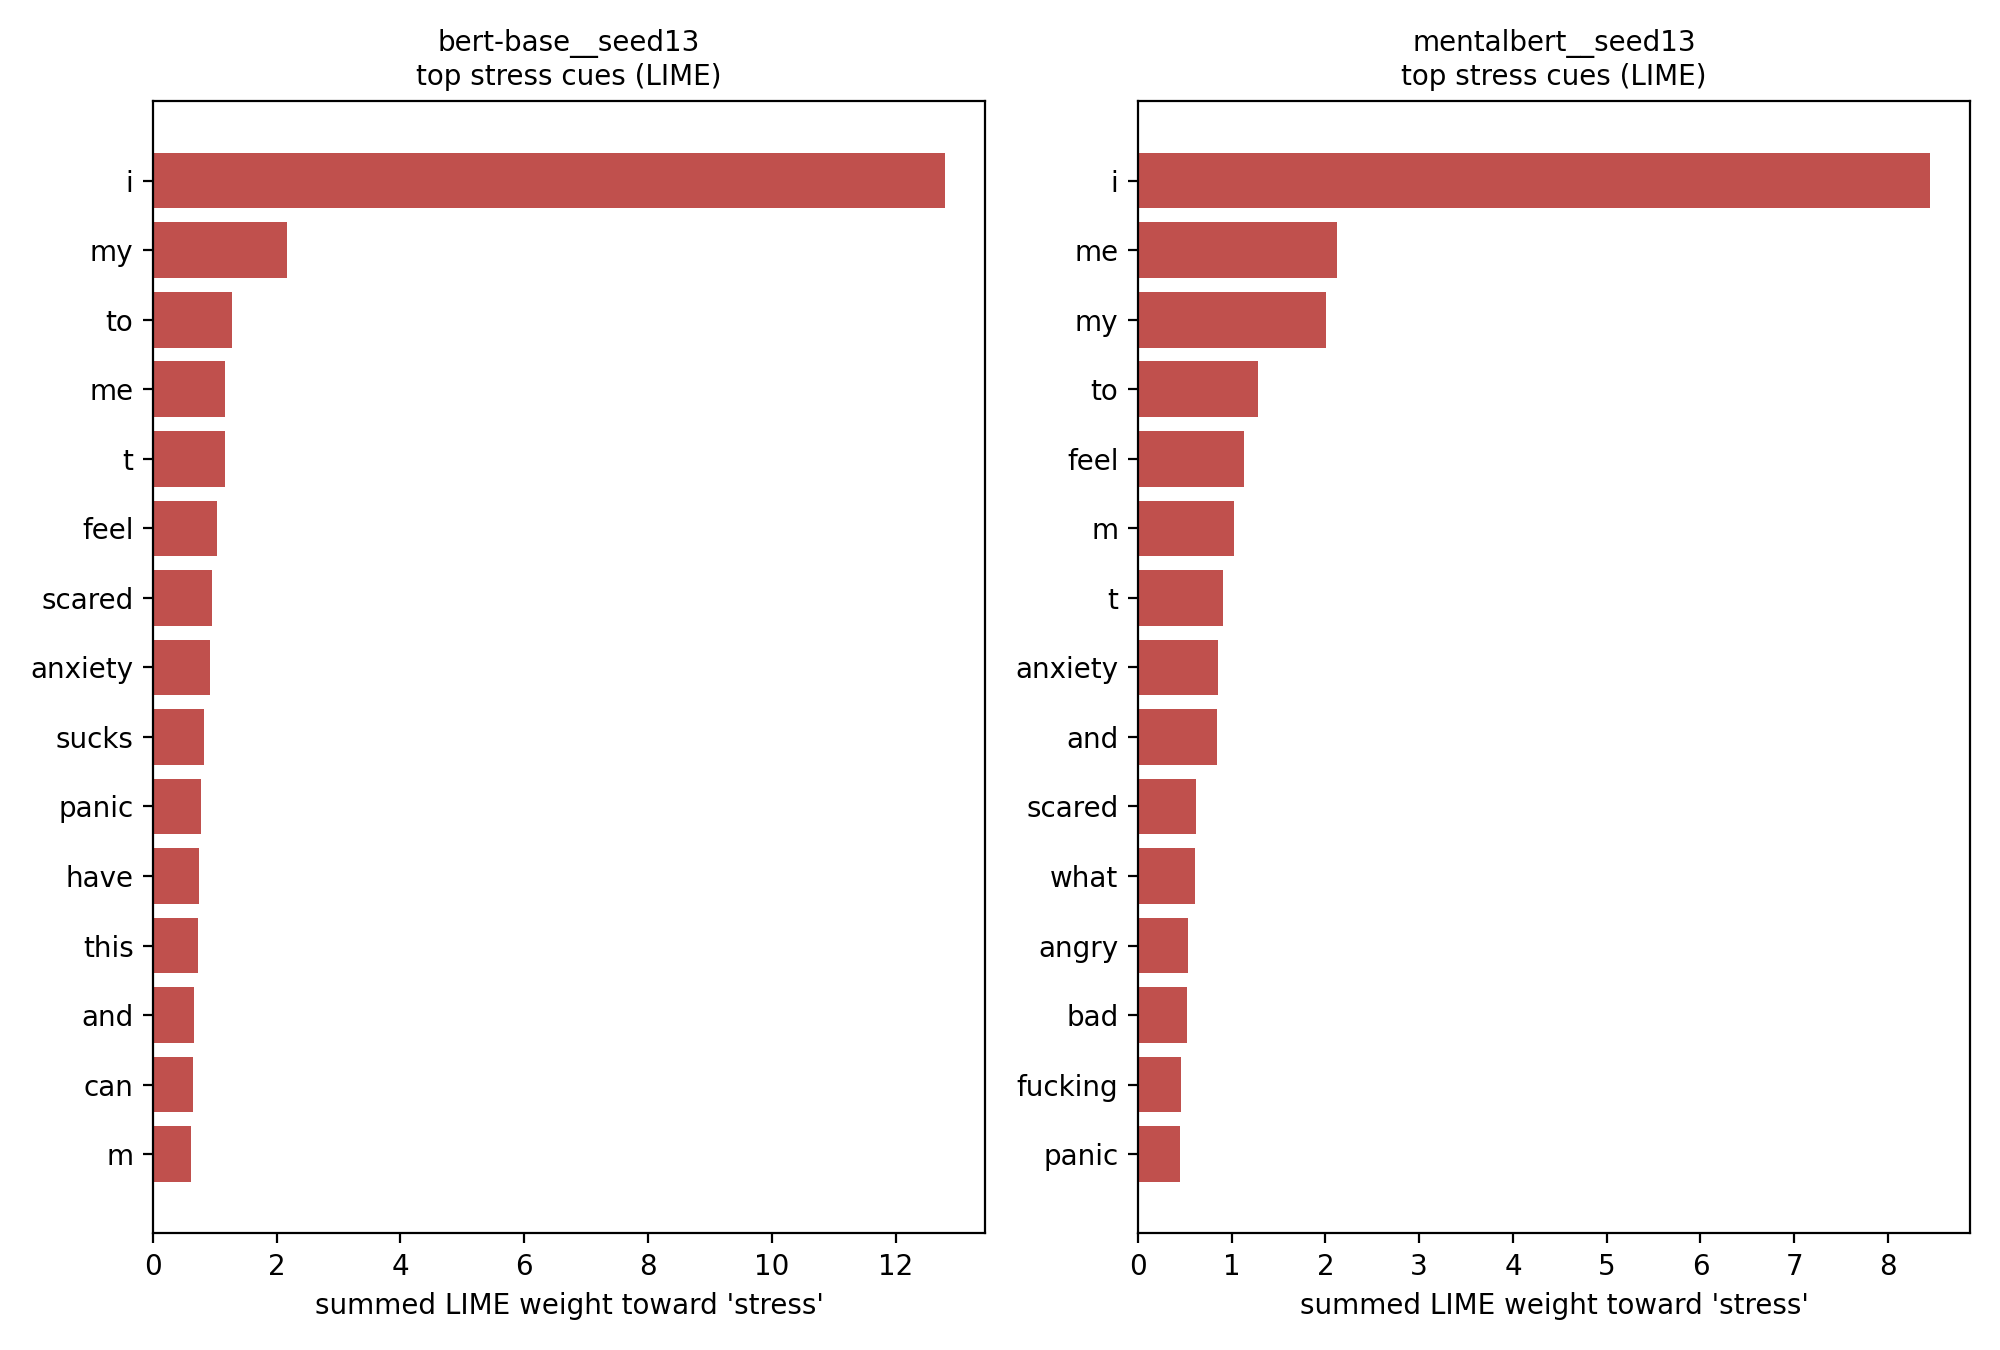
\includegraphics[width=\textwidth]{figures/lime_top_words.png}
  \caption{Words with the largest summed LIME weight towards \emph{stress} over 100 test segments,
  for BERT (left) and MentalBERT (right), seed 13. Only words occurring in at least three of the
  segments are shown.}
  \label{fig:lime}
\end{figure}

\tbd{Describe Figure~\ref{fig:lime}. Group the top cues into types: negative emotion words
(e.g.\ anxious, scared), first-person pronouns, intensifiers and negations, and topic words (money,
rent, health, partner). Which types are shared by both models and which are specific to one? Does
MentalBERT rely more on emotion and symptom words and less on topic words than BERT?}

\tbd{One or two attention heatmaps with a short comment, plus the caveat that attention is not
necessarily explanation \cite{jain2019attention}.}

\paragraph{Error analysis.}
\tbd{From results/analysis/errors\_mentalbert.csv and disagreements.csv: typical false positives
(e.g.\ posts that describe a past stressful event but in a calm tone, or posts asking for practical
help with financial vocabulary), typical false negatives (stress expressed indirectly, sarcasm,
understatement). How many segments do BERT and MentalBERT disagree on, and which one is right more
often? Relate errors to low annotator agreement where possible.}

% =====================================================================
\section{Ethical Considerations}
\label{sec:ethics}
% [Suyash + Sarthak -> Saurabh]
Detecting stress from personal writing is a sensitive application, and we discuss the main risks
following Benton {\it et al.}~\shortcite{benton2017ethical} and Chancellor {\it et al.}~\shortcite{chancellor2019taxonomy}.

\paragraph{Privacy and consent.} Dreaddit consists of public Reddit posts, but public is not the same
as consented: the authors wrote for their community, not for researchers, and many describe abuse,
trauma, homelessness or mental illness. Studies of user attitudes show that many people do not expect
their posts to be used for research and object to it in sensitive contexts \cite{fiesler2018participant}.
Although Reddit accounts are pseudonymous, a verbatim quote can be traced back to the original post
by a web search. We therefore do not redistribute any post text (our repository stores only post
identifiers and predictions), we do not attempt to identify or profile users, we report only
aggregate results, and we paraphrase rather than quote posts in this paper.

\paragraph{Errors have unequal costs.} A false negative, missing a person in distress, can mean that
help is not offered; a false positive can label someone as stressed who is not, which is intrusive
and, if acted on by others, potentially harmful. Our best model still misclassifies
\tbd{about x\%} of test segments, and the error rate differs between communities
(Section~\ref{sec:results}). The right balance between the two error types depends on how a system is
used, and it should be chosen deliberately by the people deploying it, not left at a default
threshold.

\paragraph{Not a diagnostic tool.} The labels measure whether crowd workers \emph{perceived} stress in
a five-sentence segment. This is not a clinical assessment: it says nothing about a person's health
or long-term state, and the annotators themselves often disagree (mean agreement 0.79). A model
trained on these labels inherits their noise and the annotators' own biases, and its outputs must
not be presented as a diagnosis.

\paragraph{Bias and generalisation.} Dreaddit covers ten English-language subreddits whose users are
not representative of the general population, and stress is expressed differently across cultures,
dialects, ages and genders. A model trained on it may perform worse for groups that are
under-represented or that express distress differently, and it may confuse the topic of a community
with the state of the writer (Section~\ref{sec:data}). We have not been able to measure performance
across demographic groups, since Dreaddit contains no demographic information.

\paragraph{Dual use.} The same classifier that could help a moderator prioritise posts could be used
by employers, insurers, schools or governments to monitor individuals without their knowledge and
to discriminate against them. We consider any use on individuals without their informed consent to
be a misuse of this work. Appropriate uses keep a human in the loop, such as a moderator or a
clinician who reviews flagged posts and decides what to do, are opt-in for the people being analysed,
and come with clear routes to professional help.

% =====================================================================
\section{Limitations and Future Work}
% [Saurabh -> all]
Our study has several limitations. First, the dataset is small: with 715 test segments, the 95\%
confidence interval of a macro-F1 score is several points wide, so small differences between models
are hard to establish even with significance tests. Second, the labels are assigned to five-sentence
segments, not to whole posts or to people, and are noisy, as the annotator agreement shows. Third, all
data come from one platform, in English, and from ten communities, so we cannot say how the models
behave on other platforms, languages or populations. Fourth, MentalBERT and MentalRoBERTa were
pretrained on Reddit, the same platform as Dreaddit, and possibly on some of the same communities;
part of their advantage, if any, may therefore come from familiarity with Reddit language rather
than with mental-health language in general.
% VERIFY: keep the "same communities" clause only if Ji et al.'s subreddit list overlaps with Dreaddit's.
Fifth, LLM results are sensitive to the exact prompt and to the choice of in-context examples; we
tested one prompt, one model and one example count. Finally, compute limits kept us to base-size
encoders, three seeds and a 4-bit 7B LLM, and we did not tune hyper-parameters per model.

Future work could pretrain on a broader mental-health corpus that excludes the evaluation
communities, to separate the effects of platform and domain; fine-tune the LLM with
parameter-efficient methods such as LoRA instead of only prompting it; evaluate across datasets and
platforms; and test whether explanations such as those in Section~\ref{sec:explain} actually help
human moderators make better decisions.

% =====================================================================
\section{Conclusion}
% [Suyash -> all] Fill after results. One or two sentences per RQ.
We compared a BiLSTM, general and mental-health-domain pretrained encoders, and a prompted LLM for
stress detection on Dreaddit under one shared split, evaluation pipeline and set of seeds.
\textbf{RQ1:} \tbd{does domain-adaptive pretraining help, by how much, and is it significant?}
\textbf{RQ2:} \tbd{how close does the untrained LLM come, and how much does threshold tuning or
few-shot prompting help?}
\textbf{RQ3:} \tbd{which cues the models use, and how the general and domain models differ.}
Pretrained knowledge matters at every level we tested: even for the BiLSTM, GloVe embeddings add
about four points of macro-F1. Stress classifiers remain error-prone and built on subjective labels,
so they should support, not replace, human judgement, and only with the consent of the people whose
writing is analysed.

% =====================================================================
\section*{Team Contributions}
% Check this against what actually happened before submitting.
All three authors reviewed every pull request to the repository (both non-authors approved each
change) and ran every script at least once, and each author wrote report sections outside their own
lead area.
\textbf{Suyash Yadav} led data processing, the post-grouped split, the shared evaluation and
significance-testing code, the BiLSTM baselines and the LLM experiments, and maintained the
repository, and wrote the Introduction, parts of Related Work, the encoder methods, the Experimental
Setup and the Conclusion, and co-wrote the Ethics section.
\textbf{Saurabh Bisht} led the fine-tuning of BERT, RoBERTa, MentalBERT and MentalRoBERTa and the
significance tests between them \tbd{and the TAPT experiment}, and wrote the Dataset, Results and
Limitations sections, parts of Related Work, and the methods for domain-adapted encoders and
explanations.
\textbf{Sarthak Mishra} led the LIME and attention analysis, the error analysis and the ethics
discussion, and assembled the report on Overleaf, and wrote the BiLSTM and LLM methods, the
explanation and error-analysis section, the Abstract, and co-wrote the Ethics section.

\begin{thebibliography}{}
\bibitem[\protect\citename{Benton {\it et al.}\ }2017]{benton2017ethical}
 Benton, A., Coppersmith, G. and Dredze, M. (2017) Ethical research protocols for social media health
 research. In {\it Proceedings of the First ACL Workshop on Ethics in Natural Language Processing}.
\bibitem[\protect\citename{Berg-Kirkpatrick {\it et al.}\ }2012]{berg2012empirical}
 Berg-Kirkpatrick, T., Burkett, D. and Klein, D. (2012) An empirical investigation of statistical
 significance in NLP. In {\it Proceedings of EMNLP-CoNLL}, pp.~995--1005.
\bibitem[\protect\citename{Brown {\it et al.}\ }2020]{brown2020language}
 Brown, T. B., Mann, B., Ryder, N., Subbiah, M., Kaplan, J., Dhariwal, P., {\it et al.} (2020)
 Language models are few-shot learners. In {\it Advances in Neural Information Processing Systems 33}.
\bibitem[\protect\citename{Chancellor {\it et al.}\ }2019]{chancellor2019taxonomy}
 Chancellor, S., Birnbaum, M. L., Caine, E. D., Silenzio, V. M. B. and De Choudhury, M. (2019)
 A taxonomy of ethical tensions in inferring mental health states from social media. In
 {\it Proceedings of the Conference on Fairness, Accountability, and Transparency (FAT*)}.
\bibitem[\protect\citename{Conway and O'Connor }2016]{conway2016social}
 Conway, M. and O'Connor, D. (2016) Social media, big data, and mental health: current advances and
 ethical implications. {\it Current Opinion in Psychology} {\bf 9}: 77--82.
\bibitem[\protect\citename{Coppersmith {\it et al.}\ }2014]{coppersmith2014quantifying}
 Coppersmith, G., Dredze, M. and Harman, C. (2014) Quantifying mental health signals in Twitter. In
 {\it Proceedings of the Workshop on Computational Linguistics and Clinical Psychology (CLPsych)}.
\bibitem[\protect\citename{Dettmers {\it et al.}\ }2023]{dettmers2023qlora}
 Dettmers, T., Pagnoni, A., Holtzman, A. and Zettlemoyer, L. (2023) QLoRA: efficient finetuning of
 quantized LLMs. In {\it Advances in Neural Information Processing Systems 36}.
\bibitem[\protect\citename{Devlin {\it et al.}\ }2019]{devlin2019bert}
 Devlin, J., Chang, M.-W., Lee, K. and Toutanova, K. (2019) BERT: pre-training of deep bidirectional
 transformers for language understanding. In {\it Proceedings of NAACL-HLT}.
\bibitem[\protect\citename{Dror {\it et al.}\ }2018]{dror2018hitchhiker}
 Dror, R., Baumer, G., Shlomov, S. and Reichart, R. (2018) The hitchhiker's guide to testing
 statistical significance in natural language processing. In {\it Proceedings of ACL}.
\bibitem[\protect\citename{Fiesler and Proferes }2018]{fiesler2018participant}
 Fiesler, C. and Proferes, N. (2018) ``Participant'' perceptions of Twitter research ethics.
 {\it Social Media + Society} {\bf 4}(1).
\bibitem[\protect\citename{Guntuku {\it et al.}\ }2017]{guntuku2017detecting}
 Guntuku, S. C., Yaden, D. B., Kern, M. L., Ungar, L. H. and Eichstaedt, J. C. (2017) Detecting
 depression and mental illness on social media: an integrative review. {\it Current Opinion in
 Behavioral Sciences} {\bf 18}: 43--49.
\bibitem[\protect\citename{Gururangan {\it et al.}\ }2020]{gururangan2020dont}
 Gururangan, S., Marasovi\'c, A., Swayamdipta, S., Lo, K., Beltagy, I., Downey, D. and Smith, N. A.
 (2020) Don't stop pretraining: adapt language models to domains and tasks. In {\it Proceedings of ACL}.
\bibitem[\protect\citename{Hochreiter and Schmidhuber }1997]{hochreiter1997lstm}
 Hochreiter, S. and Schmidhuber, J. (1997) Long short-term memory. {\it Neural Computation} {\bf 9}(8): 1735--1780.
\bibitem[\protect\citename{Jain and Wallace }2019]{jain2019attention}
 Jain, S. and Wallace, B. C. (2019) Attention is not explanation. In {\it Proceedings of NAACL-HLT}.
\bibitem[\protect\citename{Ji {\it et al.}\ }2022]{ji2022mentalbert}
 Ji, S., Zhang, T., Ansari, L., Fu, J., Tiwari, P. and Cambria, E. (2022) MentalBERT: publicly available
 pretrained language models for mental healthcare. In {\it Proceedings of LREC}. arXiv:2110.15621.
\bibitem[\protect\citename{Lazarus and Folkman }1984]{lazarus1984stress}
 Lazarus, R. S. and Folkman, S. (1984) {\it Stress, Appraisal, and Coping}. New York: Springer.
\bibitem[\protect\citename{Liu {\it et al.}\ }2019]{liu2019roberta}
 Liu, Y., Ott, M., Goyal, N., Du, J., Joshi, M., Chen, D., Levy, O., Lewis, M., Zettlemoyer, L. and
 Stoyanov, V. (2019) RoBERTa: a robustly optimized BERT pretraining approach. arXiv:1907.11692.
\bibitem[\protect\citename{Loshchilov and Hutter }2019]{loshchilov2019decoupled}
 Loshchilov, I. and Hutter, F. (2019) Decoupled weight decay regularization. In {\it Proceedings of
 ICLR}.
\bibitem[\protect\citename{McNemar }1947]{mcnemar1947note}
 McNemar, Q. (1947) Note on the sampling error of the difference between correlated proportions or
 percentages. {\it Psychometrika} {\bf 12}(2): 153--157.
\bibitem[\protect\citename{Pennington {\it et al.}\ }2014]{pennington2014glove}
 Pennington, J., Socher, R. and Manning, C. D. (2014) GloVe: global vectors for word representation.
 In {\it Proceedings of EMNLP}.
\bibitem[\protect\citename{Qwen Team }2024]{qwen2024qwen25}
 Qwen Team (2024) Qwen2.5 technical report. arXiv:2412.15115.
\bibitem[\protect\citename{Ribeiro {\it et al.}\ }2016]{ribeiro2016lime}
 Ribeiro, M. T., Singh, S. and Guestrin, C. (2016) ``Why should I trust you?'': explaining the
 predictions of any classifier. In {\it Proceedings of ACM SIGKDD}.
\bibitem[\protect\citename{Turcan and McKeown }2019]{turcan2019dreaddit}
 Turcan, E. and McKeown, K. (2019) Dreaddit: a Reddit dataset for stress analysis in social media.
 In {\it Proceedings of the 10th International Workshop on Health Text Mining and Information
 Analysis (LOUHI)}. arXiv:1911.00133.
\bibitem[\protect\citename{Wiegreffe and Pinter }2019]{wiegreffe2019attention}
 Wiegreffe, S. and Pinter, Y. (2019) Attention is not not explanation. In {\it Proceedings of
 EMNLP-IJCNLP}.
\bibitem[\protect\citename{Xu {\it et al.}\ }2024]{xu2024mentalllm}
 Xu, X., Yao, B., Dong, Y., Gabriel, S., Yu, H., Hendler, J., Ghassemi, M., Dey, A. K. and Wang, D.
 (2024) Mental-LLM: leveraging large language models for mental health prediction via online text
 data. {\it Proceedings of the ACM on Interactive, Mobile, Wearable and Ubiquitous Technologies} {\bf 8}(1).
\bibitem[\protect\citename{Yang {\it et al.}\ }2023]{yang2023towards}
 Yang, K., Ji, S., Zhang, T., Xie, Q., Kuang, Z. and Ananiadou, S. (2023) Towards interpretable mental
 health analysis with large language models. In {\it Proceedings of EMNLP}.
\end{thebibliography}

\label{lastpage}
\end{document}
